
\begin{figure}
\center

	\begin{subfigure}[t]{0.22\textwidth}
		\center
		
\includegraphics[width=\textwidth]{images/findings/experiments/regularization/strats/0.50/hand_max_min.png}
		\caption{\handmaxmin}
	\end{subfigure}
	~
	\begin{subfigure}[t]{0.22\textwidth}
		\center
		
\includegraphics[width=\textwidth]{images/findings/experiments/regularization/strats/0.50/hand_max_avg.png}
		\caption{\handmaxavg}
	\end{subfigure}
~
	\begin{subfigure}[t]{0.22\textwidth}
		\center
		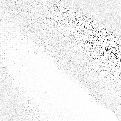
\includegraphics[width=\textwidth]{images/findings/experiments/regularization/strats/0.50/hand_max_med.png}
		\caption{\handmaxmed}
	\end{subfigure}
	~
	\begin{subfigure}[t]{0.22\textwidth}
		\center
		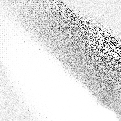
\includegraphics[width=\textwidth]{images/findings/experiments/regularization/strats/0.50/hand_max_poss.png}
		\caption{\handmaxposs}
	\end{subfigure}

	\begin{subfigure}[t]{0.22\textwidth}
		\center
		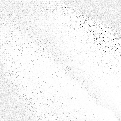
\includegraphics[width=\textwidth]{images/findings/experiments/regularization/strats/0.50/crib_min_avg.png}
		\caption{\cribminavg}
	\end{subfigure}
	~
	\begin{subfigure}[t]{0.22\textwidth}
		\center
		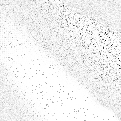
\includegraphics[width=\textwidth]{images/findings/experiments/regularization/strats/0.50/pegging_max_avg_gained.png}
		\caption{\peggingmaxavggained}
	\end{subfigure}
~
	\begin{subfigure}[t]{0.22\textwidth}
		\center
		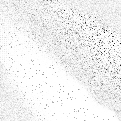
\includegraphics[width=\textwidth]{images/findings/experiments/regularization/strats/0.50/pegging_max_med_gained.png}
		\caption{\peggingmaxmedgained}
	\end{subfigure}
	~
	\begin{subfigure}[t]{0.22\textwidth}
		\center
		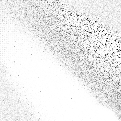
\includegraphics[width=\textwidth]{images/findings/experiments/regularization/strats/0.50/pegging_min_avg_given.png}
		\caption{\peggingminavggiven}
	\end{subfigure}

\caption{
	Final strategies for an agent using regularized learning
	when playing as the dealer
	and the maximum value weight allowed is 0.50
	after training for 500,000 games.
}
\label{fig:reg-strats-0.50}
\end{figure}
